\documentclass[a4paper,
fontsize=11pt,
%headings=small,
oneside,
numbers=noperiodatend,
parskip=half-,
bibliography=totoc,
final
]{scrartcl}

\usepackage{synttree}
\usepackage{graphicx}
\setkeys{Gin}{width=.4\textwidth} %default pics size

\graphicspath{{./plots/}}
\usepackage[ngerman]{babel}
\usepackage[T1]{fontenc}
%\usepackage{amsmath}
\usepackage[utf8x]{inputenc}
\usepackage [hyphens]{url}
\usepackage{booktabs} 
\usepackage[left=2.4cm,right=2.4cm,top=2.3cm,bottom=2cm,includeheadfoot]{geometry}
\usepackage{eurosym}
\usepackage{multirow}
\usepackage[ngerman]{varioref}
\setcapindent{1em}
\renewcommand{\labelitemi}{--}
\usepackage{paralist}
\usepackage{pdfpages}
\usepackage{lscape}
\usepackage{float}
\usepackage{acronym}
\usepackage{eurosym}
\usepackage[babel]{csquotes}
\usepackage{longtable,lscape}
\usepackage{mathpazo}
\usepackage[normalem]{ulem} %emphasize weiterhin kursiv
\usepackage[flushmargin,ragged]{footmisc} % left align footnote
\usepackage{ccicons} 

%%%% fancy LIBREAS URL color 
\usepackage{xcolor}
\definecolor{libreas}{RGB}{112,0,0}

\usepackage{listings}

\urlstyle{same}  % don't use monospace font for urls

\usepackage[fleqn]{amsmath}

%adjust fontsize for part

\usepackage{sectsty}
\partfont{\large}

%Das BibTeX-Zeichen mit \BibTeX setzen:
\def\symbol#1{\char #1\relax}
\def\bsl{{\tt\symbol{'134}}}
\def\BibTeX{{\rm B\kern-.05em{\sc i\kern-.025em b}\kern-.08em
    T\kern-.1667em\lower.7ex\hbox{E}\kern-.125emX}}

\usepackage{fancyhdr}
\fancyhf{}
\pagestyle{fancyplain}
\fancyhead[R]{\thepage}

% make sure bookmarks are created eventough sections are not numbered!
% uncommend if sections are numbered (bookmarks created by default)
\makeatletter
\renewcommand\@seccntformat[1]{}
\makeatother


\usepackage{hyperxmp}
\usepackage[colorlinks, linkcolor=black,citecolor=black, urlcolor=libreas,
breaklinks= true,bookmarks=true,bookmarksopen=true]{hyperref}
%URLs hart brechen
\makeatletter 
\g@addto@macro\UrlBreaks{ 
  \do\a\do\b\do\c\do\d\do\e\do\f\do\g\do\h\do\i\do\j 
  \do\k\do\l\do\m\do\n\do\o\do\p\do\q\do\r\do\s\do\t 
  \do\u\do\v\do\w\do\x\do\y\do\z\do\&\do\1\do\2\do\3 
  \do\4\do\5\do\6\do\7\do\8\do\9\do\0} 
% \def\do@url@hyp{\do\-} 
\makeatother 

%meta
%meta

\fancyhead[L]{Redaktion LIBREAS \\ %author
LIBREAS. Library Ideas, 33 (2018). % journal, issue, volume.
\href{http://nbn-resolving.de/}
{}} % urn 
% recommended use
%\href{http://nbn-resolving.de/}{\color{black}{urn:nbn:de...}}
\fancyhead[R]{\thepage} %page number
\fancyfoot[L] {\ccLogo \ccAttribution\ \href{https://creativecommons.org/licenses/by/3.0/}{\color{black}Creative Commons BY 3.0}}  %licence
\fancyfoot[R] {ISSN: 1860-7950}

\title{\LARGE{Editorial \#33: Ortstermin. Reportagen aus der tatsächlichen Bibliotheksarbeit}} % title
\author{Redaktion LIBREAS} % author

\setcounter{page}{1}

\hypersetup{%
      pdftitle={Editorial \#33: Ortstermin. Reportagen aus der tatsächlichen Bibliotheksarbeit},
      pdfauthor={Readktion LIBREAS},
      pdfcopyright={CC BY 3.0 Unported},
      pdfsubject={LIBREAS. Library Ideas, 33 (2018).},
      pdfkeywords={Bibliothek, Berufspraxis},
      pdflicenseurl={https://creativecommons.org/licenses/by/3.0/},
      pdfcontacturl={http://libreas.eu},
      baseurl={http://libreas.eu},
      pdflang={de},
      pdfmetalang={de}
     }



\date{}
\begin{document}

\maketitle
\thispagestyle{fancyplain} 

%abstracts

%body
Ein Editorial kann, sollte sogar, eine Geschichte über das Entstehen der
jeweiligen Zeitschriftennummer sein. Insoweit: Die Idee zu dieser
Ausgabe entstand, weil wir selber oft Bibliotheken besuchen (wie so
viele andere Kolleginnen und Kollegen auch): regelmäßig zum Arbeiten, im
Urlaub, auf Kurztrips, bei Weiterbildungs- und Konferenzbesuchen oder
einfach mal so, aus reiner Neugier. Wir treffen bei solchen Besuchen
eigentlich immer engagierte Kolleginnen und Kollegen, die gern durch ihr
Haus führen oder von ihrem Alltag berichten. Gute Bildmotive finden sich
auch. Aber auffällig ist, was stolz gezeigt wird: Die Probleme, von
denen man berichtet oder auch der Alltag, den man einfach sieht --
Familien, die vorbei kommen, die Menschen, welche die Bibliothek einfach
nutzen, so als ob sie es schon immer taten, Jugendliche und Studierende,
die ruhig vor sich hinlernen -- wirken eigentlich immer etwas anders,
als die Bilder, die man in der bibliothekarischen Literatur findet. Zum
Beispiel sind die meisten Bibliotheken sehr, sehr ruhig, aber doch
belebt; nicht, wie es in der Literatur den Eindruck hat, entweder leer
oder durch neue Angebote ständig voll und laut. Ein anderes Beispiel:
Die Ausstattung der meisten Bibliotheken ist gar nicht so neu, wie es
auf den Werbeanzeigen der Bibliotheksausstatter erscheint, aber auch
nicht gänzlich kaputt. Meistens scheint es in einem Zwischenstatus zu
sein: Gebraucht, aber noch nicht unbrauchbar. Dies aufzugreifen und
einen unmittelbaren Blick auf und in Bibliotheken zu werfen lag also
nah. Um es aufzugreifen bedurfte es freilich eines Impulses.

Dieser ergab sich aus einem eigentlich nicht-bibliothekarischen Ausflug.
Konkret verschlug es einige Redakteurinnen und Redakteure (zusammen mit
anderen) nach Berlin, Bezirk Marzahn-Hellersdorf zum \enquote{Acht Tage
Marzahn}-Kunstfestival.\footnote{\url{http://www.acht-tage-marzahn.de/}}
Dieses hatte einige Schaucontainer vor dem Freizeitforum Marzahn
platziert, in dem sich neben einer Schwimmhalle und Veranstaltungsräumen
eben auch die -- übrigens sehr sehenswerte -- Mark-Twain-Bibliothek
befindet. Daran vorbeizugehen war erwartungsgemäß nicht möglich.

\begin{figure}
\centering
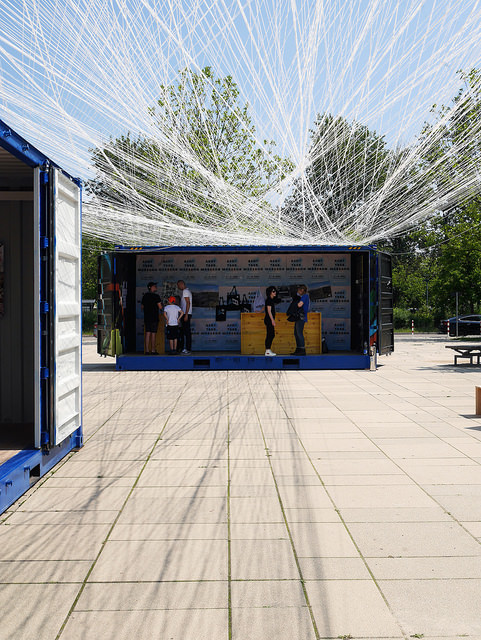
\includegraphics{image_1.jpg}
\caption{Redaktionsorte XII: Berlin Marzahn (Veranstaltungsort Acht Tage
Marzahn, Juli 2017, Victor-Klemperer-Platz in Berlin-Marzahn. Zugleich:
Ein ganz normaler sommerlicher Redaktionsort. Quelle:
\url{https://www.flickr.com/photos/benkaden/35651455301/}) Foto: Ben
Kaden, CC-BY 2.0)}
\end{figure}

Dieser Besuch regte nun dazu an, sich mehr Reportagen, mehr Erzählung,
mehr Bilder aus dem Alltag der Bibliotheken zu wünschen. Es fiel nicht
schwer, den Rest der Redaktion von diesem Wunsch zu überzeugen, auch der
Call for Papers kam gut an. Die Rückmeldungen waren positiv. Ein
Bibliotheksdirektor vermutete sogar, dass viele Kolleginnen und Kollegen
die Möglichkeit nutzen würden, um sich über die Leitungen ihrer
Bibliotheken zu beschweren. (Das ist nicht passiert.) Weil wir möglichst
viel hören, sehen, erfahren wollten, versuchten wir, die
Einstiegsschwellen noch niedriger zu gestalten als sonst. Die Idee, eine
Umfrage zu gestalten wurde uns von Leslie Kuo\footnote{\url{https://twitter.com/leslie_kuo}}
bei ihrem Besuch auf einer unserer Redaktionssitzungen angetragen und
quasi sofort umgesetzt. Es ist die bislang niedrigschwelligste Form, an
der LIBREAS mitzuwirken.

Bei jedem unserer Calls müssen wir damit umgehen, dass sie nicht so
funktionieren, wie wir es uns erhoffen. Diesmal wollten wir Hunderte von
Berichten und das ist nicht passiert. Aber gleichzeitig entsteht immer
wieder eine Ausgabe. Wir erhielten auf unsere Umfrage immerhin 15
Antworten, die Einblick in sehr unterschiedliche Bibliotheken
ermöglichen. Das ist gut, auch wenn wir außerordentlich gern noch von
weiteren Bibliotheken gehört hätten. Die Artikel, die uns erreichten,
zeigen auch das, was wir bei Besuchen immer wieder sehen: Engagierte
Kolleginnen und Kollegen, die sich mit anderen Herausforderungen und
Möglichkeiten auseinandersetzen, als es die bibliothekarische Literatur
vermuten lässt. Das wir so eine Diversität abbilden können -- One Person
Libraries, Öffentliche Bibliothek kleinerer Gemeinden und großer Städte,
grössere Wissenschaftliche Bibliotheken, aus Deutschland, Österreich,
der Schweiz und Brasilien -- freut uns. Dass es sich anbietet, den
Ortstermin als offene Rubrik zukünftig mit der Zeitschrift weiterlaufen
zu lassen, liegt auf der Hand.

Es fällt, wenig überraschend, auf, dass gerade in den kleineren
Bibliotheken ein Großteil der Herausforderungen auf ein bestimmtes
Problem zurückgeführt werden kann: Geld, genauer zu wenig Geld und damit
auch zu wenig Personal, zu wenig Infrastruktur, zu wenig
Zukunftssicherheit. Das ist auf der einen Seite nicht unerwartet, auf
der anderen Seite aber auch bezeichnend: Ein Blick in die
bibliothekarische Literatur zeigt diese Herausforderung eigentlich
nicht. Dort finden sich eher Projekte und Angebote repräsentiert, die
schon finanziert sind. Meist sind dies Projekte und Angebote größerer
Bibliotheken, solcher mit besserem Zugang zu Etat und
Fördermöglichkeiten.

Ein Editorial ist kein Platz für lange Debatten, aber uns scheint, dass
es sinnvoll wäre, wenn das Bibliothekswesen -- oder Teile davon, zum
Beispiel die bibliothekarischen Verbände DBV, VDB, BVÖ, VÖB, der neu
gebildete Bibliosuisse oder auch Vereine wie unser eigener LIBREAS.
Verein -- sich auch um diese sehr spürbare Lücke zwischen Leuchttürmen
und den Wellengängen des Alltags kümmern würde. Die Lage scheint sich
zwar im Vergleich zu den großen Brüchen der vergangenen Jahrzehnte
leicht zu verbessern. Aber gerade im kommunalen Bereich sind es eben oft
auch Einspar-wellen, die die Bibliotheken daran hindern, bei den jeweils
aktuellen Gegenwarts- und Zukunftstrends mitzusegeln. Innovation,
permanente Weiterentwicklung und politische Verankerung von Bibliotheken
sind alles wichtige Themen. Aber sie sind nicht alles. Der Alltag in den
Bibliotheken ist oft von wenig aufregenden lokalen Gegebenheiten, viel
zu regelmäßig von Geldsorgen sowie zum Glück auch von weniger
spektakulären, aber dennoch sehr wirksamen Erfolgen geprägt. Wenn wir
wissen wollen -- und um als Bibliothekswesen handeln zu können, wäre es
sinnvoll, es zu wissen --, sollten wir mehr Reportagen aus dem
Bibliotheksalltag lesen (und erstellen, als Text, als Bild, als Video,
als Vortrag oder anders). Der überwiegende Teil der Bibliotheken muss
sich nämlich nicht auf den Zukunftssessions von Bibliothekartagen und
Digitalkonferenzen beweisen. Sondern im Funktionieren im Alltag.

So oder so hoffen wir, dass auch diese Ausgabe mit Interesse gelesen
wird. Neben den Ortsterminen gibt es natürlich weitere Beiträge, die
wunderbarerweise auch sehr deutlich in Richtung tatsächlichen Diskurs
streben, unter anderem über die mögliche Arbeit von Bibliotheken in
Nunavut, Kanada. Ebenso veröffentlichen wir unsere (nicht nur)
redaktionelle Literaturrundschau \enquote{Das liest die LIBREAS}. Diese
bietet eine weitere Möglichkeit, sich einzubringen. Wer das Format
überzeugend findet, kann seine eigenen Lektüreeindrücke, die bewusst in
der Tradition des Kurzreferats stehen sollen, gern an die Redaktion per
E-Mail
\href{mailto:redaktion@libreas.eu}{\nolinkurl{redaktion@libreas.eu}}
senden.

Wer dazu oder zu anderen Aspekten rund um LIBREAS den persönlichen
Austausch sucht, ist übrigens herzlich zum
LIBREAS-Bibliothekstags-Beisammensein auf dem Bibliothekstag im Juni
2018 eingeladen.\footnote{\url{https://twitter.com/karstens/status/976080585067245568}}

Ihre / Eure Redaktion LIBREAS

(Berlin, Chur, Dresden, Göttingen)

%autor

\end{document}
